\chapter{Opzetten van de Cassandra cluster}
\label{ch:cassandra_cluster}

\section{Apache Cassandra}
Om te beginnen aan het opzetten van de van de clusters werd geopteerd om gebruik te maken van virtuele machines, die geconfigureerd werden met Vagrant.

In een eerste poging om een werkende Cassandra cluster te bekomen werd er op elke Vagrant machine Cassandra 3.3, op moment van schrijven de meest recente versie, geïnstalleerd.
Nadat dit was gebeurd dienden nog enkele stappen te voltooid worden \citep{DataStax2016}.
Deze configuratie op deze manier gaf echter veel problemen, Cassandra werd telkens na enkele bewerkingen onbruikbaar met de foutboodschap "could not access pidfile for Cassandra".
Een eerste oplossing voor dit probleem was om te zorgen dat de user cassandra toegang had tot de pidfile, want namelijk niet het geval was doordat de installatie van Cassandra werd uitgevoerd door de vagrant setup.
Maar ook dit leverde weinig resultaat op.

\section{DataStax OpsCenter}

Uiteindelijk werd er geopteerd om gebruik te maken van OpsCenter omdat dit een gemakkelijke manier is om snel een Cassandra cluster te bekomen en omdat dit ook goede mogelijkheden tot monitoren van de database voorziet.
Van het OpsCenter werd er voor de community edition 5.2.4 gekozen.
Hiermee komt Cassandra 2.1.11 geïnstalleerd \citep{Cantoni2016}.

De setup bestaat uit 1 master node waarop het OpsCenter runt en dan 3 slave nodes waar de uiteindelijke Cassandra database op komt te runnen.
Na de NAT router van Oracle Virtual Box werd een privaat netwerk opgezet zodanig deze machines met elkaar konden communiceren.
Hiervoor moest elke machine een ip-adres krijgen binnen het netwerk en ook de /etc/hosts aangepast worden.

Eenmaal de virtuele machines correct geconfigureerd waren, werd er overgegaan tot de eigenlijke installatie van Cassandra.
Zoals eerder vermeld werd hiervoor gebruik gemaakt van het OpsCenter.
Hiervoor werd op de master node naar de localhost:8888 gesurft om de installatie te starten. Op de pagina dit te voorschijn komt werd voor de optie 'brand new cluster gekozen'.

In het volgende venster wordt er om verschillende zaken gevraagd.
Tabel \ref{tab:cas_conf} en figuur \ref{fig:cas_conf_1} geven weer hoe dit venster ingevuld werd.

\begin{table}[H]
  \begin{tabular}{|l|l|}
  \hline
  Property Name & Waarde \\
  \hline
  \hline
  Cluster Name & BP Cluster \\
  \hline
  Type & local \\
  \hline
  Package & datastax community 2.1.11 \\
  \hline
  Enpoint Snitch & GossipingPropertyFileSnitch \\
  \hline
  Username en password & vagrant/vagrant\\
  \hline
  Local Node Credentials & cassandra-node-1, cassandra-node-2, cassandra-node-3 \\
  \hline
  \end{tabular}
  \caption{Configuratie van de Cassandra Cluster}
  \label{tab:cas_conf}
\end{table}

\begin{figure}[H]
  	\centering
    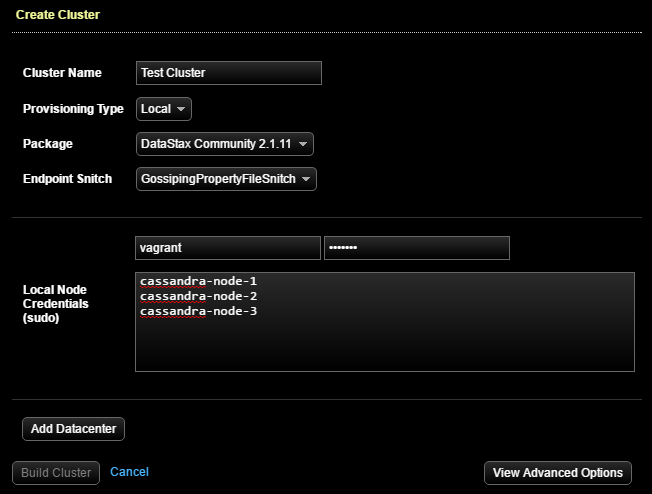
\includegraphics[width=0.5\textwidth]{img/4_installatie_cassandra/1_Configuration_part_1}
    \caption{Cassandra: Instellingen deel 1}
    \label{fig:cas_conf_1}
\end{figure}

Hier dient een datacenter toegevoegd te worden.
Hierbij wordt de naam van het datacenter vrij gekozen en zijn de node properties het ip-adres van de slave nodes (Figuur: \ref{fig:cas_conf_2}).

\begin{figure}[H]
  	\centering
    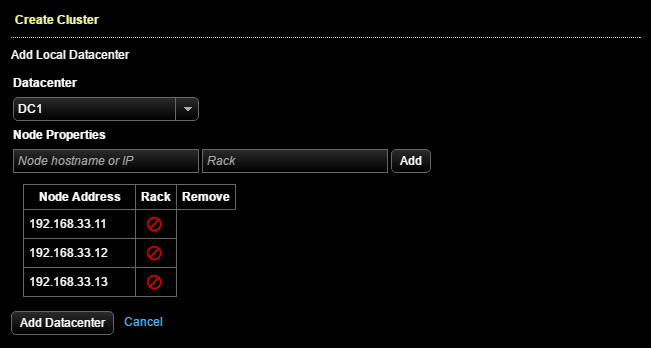
\includegraphics[width=0.5\textwidth]{img/4_installatie_cassandra/1_Configuration_part_2}
    \caption{Cassandra: Instellingen deel 2}
    \label{fig:cas_conf_2}
\end{figure}

Eenmaal de datacenters zijn toegevoegd kan men verdergaan.
Bij het drukken op de knop 'build cluster word nog gevraagd om de fingerprints van de nodes te accepteren.

Hierna begint OpsCenter met de installatie van de Cassandra cluster (Figuur: \ref{fig:cas_install}).
Deze installatie neemt enkele ogenblikken in beslag.
Als hier fouten voorkomen ligt dit veelal aan het feit dat er onvoldoende werkgeheugen aanwezig is op de slave nodes.
In de setup die hier gebruikt werd het minimum aanvaarde geheugen geven aan de slave nodes, nl 2GB.
Samen met Cassandra wordt ook de DataStax agent meegeïnstalleerd zodat het OpsCenter kan communiceren met iedere node.

\begin{figure}[H]
	\centering
	\begin{subfigure}{.49\textwidth}
  		\centering
  		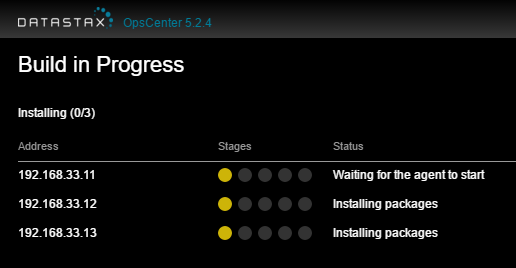
\includegraphics[width=.9\linewidth]{img/4_installatie_cassandra/1_Configuration_part_4}
  		\caption{Deel 1}
	\end{subfigure}
	\begin{subfigure}{.49\textwidth}
  		\centering
  		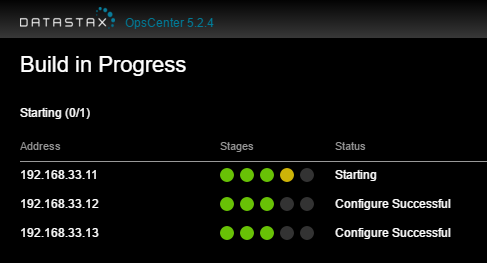
\includegraphics[width=.9\linewidth]{img/4_installatie_cassandra/1_Configuration_part_5}
  		\caption{Deel 2}
	\end{subfigure}
	\begin{subfigure}{.49\textwidth}
  		\centering
  		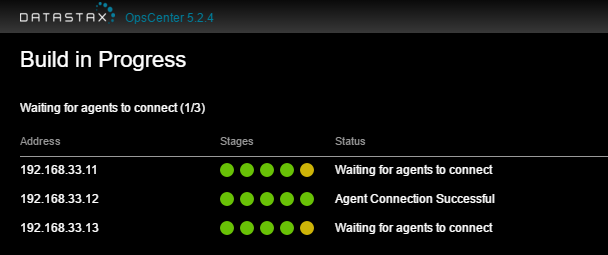
\includegraphics[width=.9\linewidth]{img/4_installatie_cassandra/1_Configuration_part_6}
  		\caption{Deel 3}
	\end{subfigure}
	\caption{Installatie van Cassandra door OpsCenter}
	\label{fig:cas_install}
\end{figure}

Na de installatie komt men terecht in het Dashboard van OpsCenter (Figuur \ref{fig:cas_opscenter_tour_dashboard}).
Hierin worden een aantal zaken weergegeven zoals de gezondheid van de cluster, het aantal write requests, de write request latency, \ldots
Hier kunnen nog meer grafieken aan toegevoegd worden via de knop "add graph".
In het tabblad nodes kan gezondheid van de cluster bekeken worden evenals hoe de data verdeeld zit over de cluster.
Deze informatie kan in ringvorm zoals op figuur \ref{fig:cas_opscenter_tour_nodes} weergegeven worden of in een lijst.

\begin{figure}[H]
	\centering
	\begin{subfigure}{.49\textwidth}
		\centering
		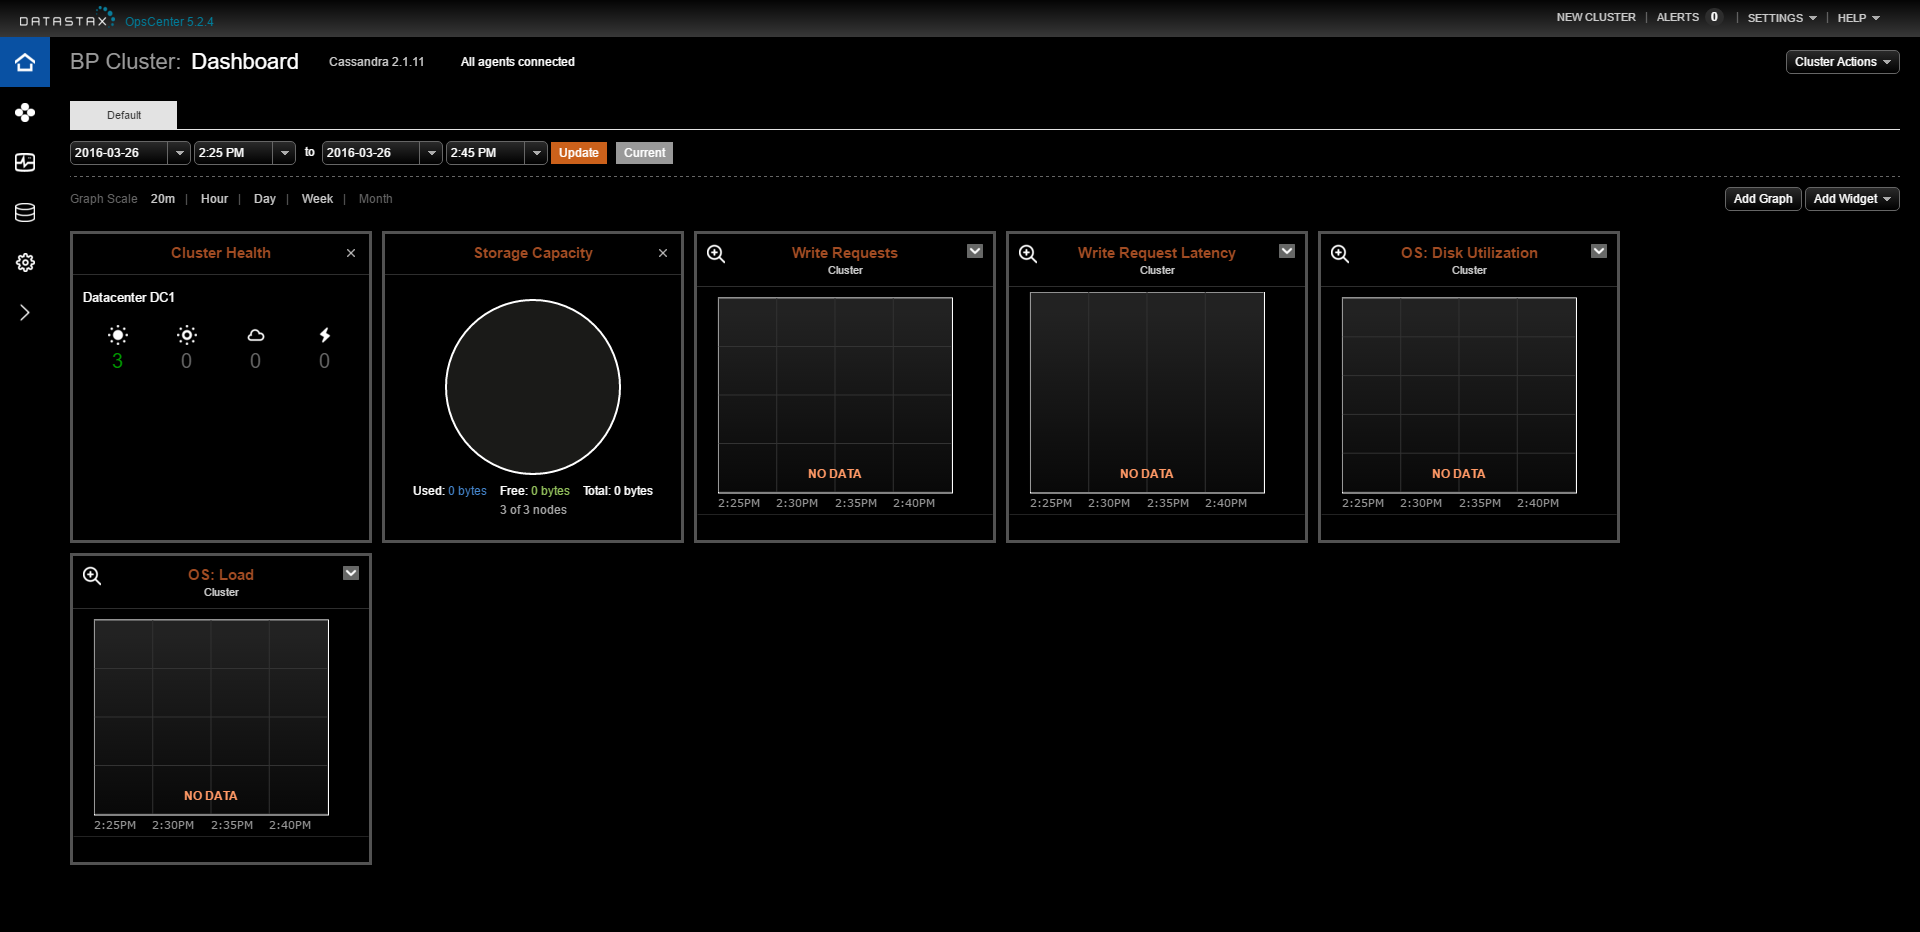
\includegraphics[width=.99\linewidth]{img/4_installatie_cassandra/2_Tour_1_Dashboard}
		\caption{Tabblad dashboard}
		\label{fig:cas_opscenter_tour_dashboard}
	\end{subfigure}
	\begin{subfigure}{.49\textwidth}
		\centering
		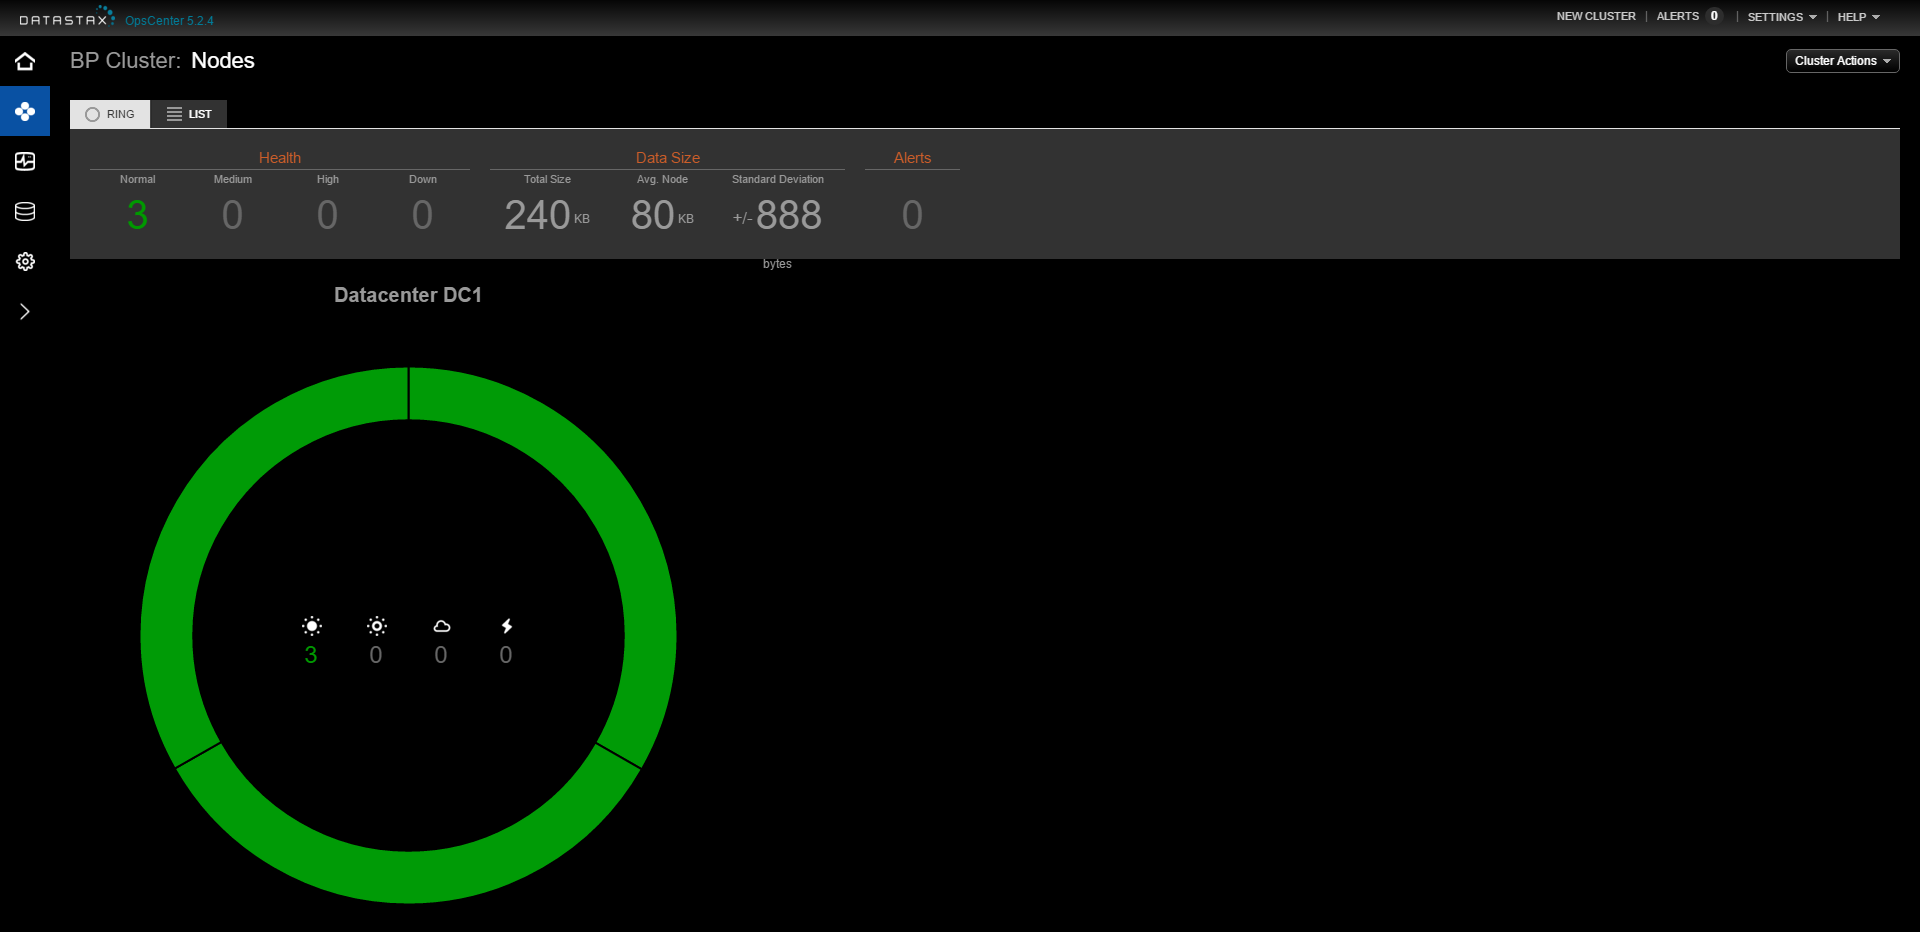
\includegraphics[width=.99\linewidth]{img/4_installatie_cassandra/2_Tour_2_Nodes}
		\caption{Tabblad nodes: ring}
		\label{fig:cas_opscenter_tour_nodes}
	\end{subfigure}
	\caption{Rondleiding in OpsCenter}
	\label{fig:cas_opscenter_tour}
\end{figure}

Cassandra voorziet zelf ook een tool die deze monitoring voorziet, nodetool.
Om te bekijken of de installatie gelukt is kan men via ssh inloggen op een van de nodes van de cluster en hier nodetool laten lopen (Figuur \ref{fig:cas_nodetool}).
Als men met nodetool de status opvraagt dan krijgt men eveneens alle nodes in de cluster te zien, samen het de hoeveelheid data die ze bevatten en hoeveel dit percentueel is van de data die aanwezig is in de cluster.

\begin{figure}[H]
	\centering
	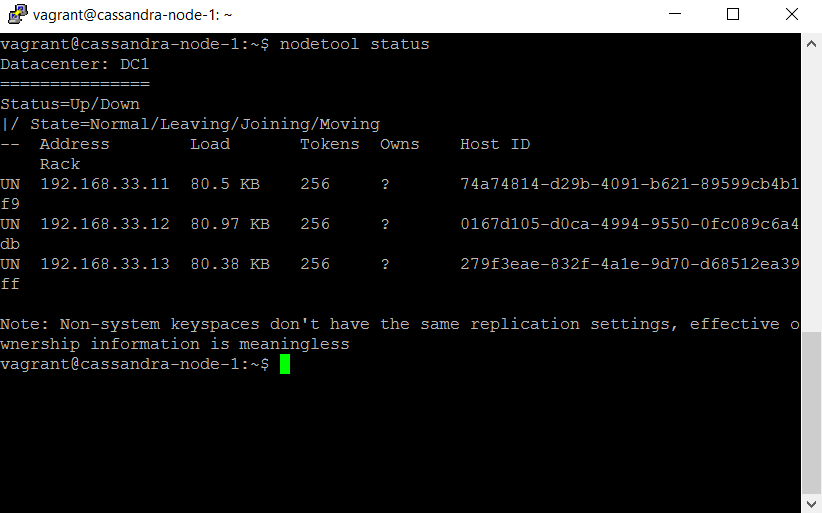
\includegraphics[width=0.5\textwidth]{img/4_installatie_cassandra/3_Node_setup}
	\caption{Nodetool}
	\label{fig:cas_nodetool}
\end{figure}

\section{Toevoegen van een node}
Het proces van het toevoegen van een node is zeer gelijkaardig aan het opzetten van de cluster.
Hierbij dient men in het OpsCenter bij het menu "cluster actions" voor de optie "add node" kiezen (Figuur \ref{fig:cas_add_node_1}).
Hier wordt een vierde node toegevoegd aan de cluster.
Net zoals bij de installatie van de cluster wordt opnieuw het scherm getoond waarin de aanmeld gegevens voor de gegeven node gevraagd worden (Figuur \ref{fig:cas_add_node_2}).
Via de knop "Add/Expand Datacenter" kan men op dezelfde manier nodes toevoegen aan het bestaande datacenter die tijdens de installatie werd aangemaakt.
Bij het bevestigen wordt opnieuw gevraagd om de fingerprint van de node te accepteren.
Hierna begint de installatie van de software op de node, de agent en cassandra worden geïnstalleerd en geconfigureerd.
Na dit alles kan men in het tabblad nodes, deze maal als een lijst, zien dat de nieuwe node is toegevoegd aan de cluster (Figuur: \ref{fig:cas_add_node_3}).

\begin{figure}[H]
	\centering
	\begin{subfigure}{.49\textwidth}
		\centering
		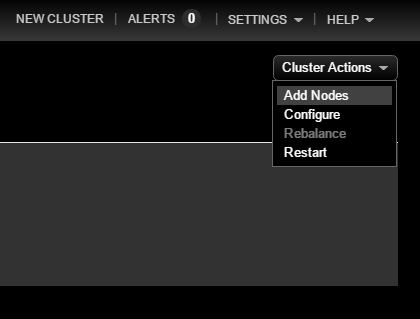
\includegraphics[width=.9\linewidth]{img/4_installatie_cassandra/4_Add_Node_1}
		\caption{Add node}
		\label{fig:cas_add_node_1}
	\end{subfigure}
	\begin{subfigure}{.49\textwidth}
		\centering
		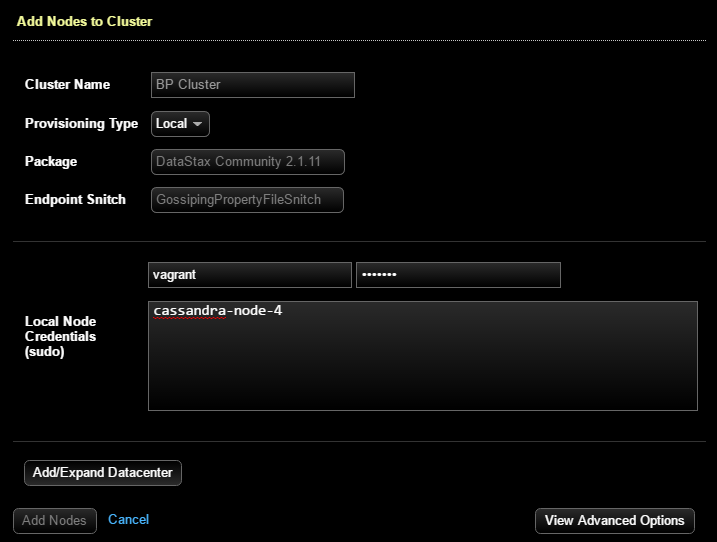
\includegraphics[width=.9\linewidth]{img/4_installatie_cassandra/4_Add_Node_2}
		\caption{Deel 2}
		\label{fig:cas_add_node_2}
	\end{subfigure}
	\begin{subfigure}{\textwidth}
		\centering
		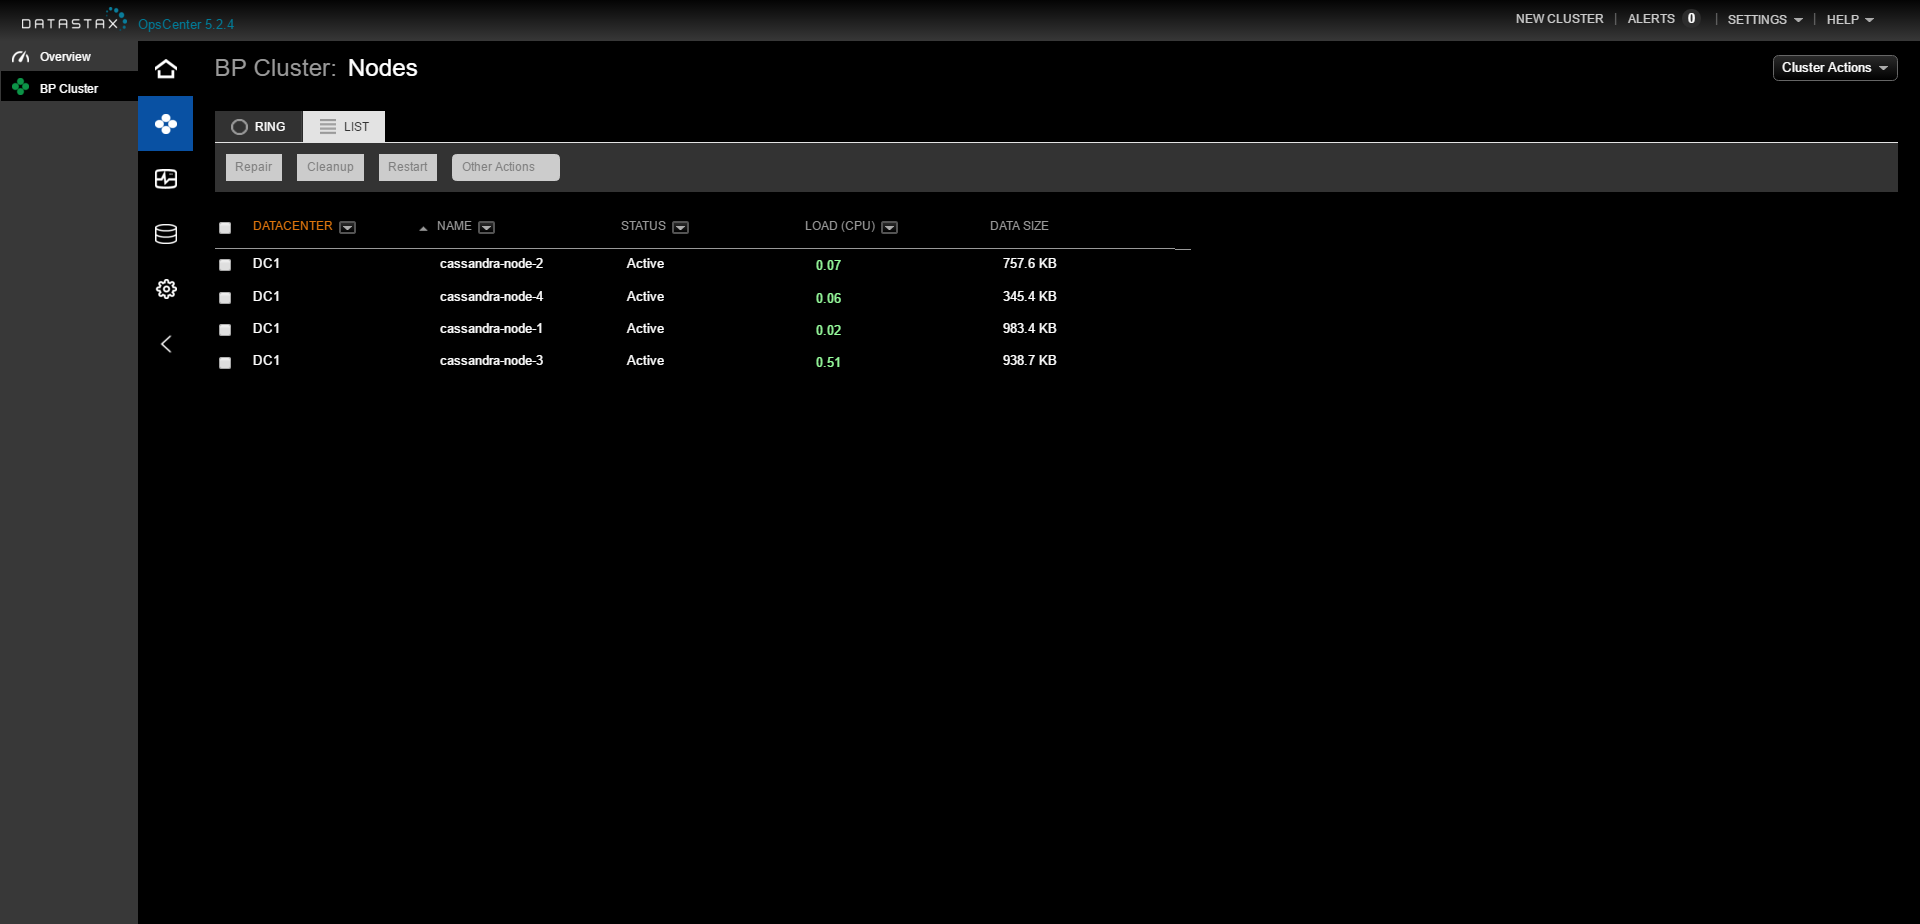
\includegraphics[width=.9\linewidth]{img/4_installatie_cassandra/4_Add_Node_7a}
		\caption{Tabblad node met 4 nodes}
		\label{fig:cas_add_node_3}
	\end{subfigure}
	\caption{Toevoegen van een node via OpsCenter}
	\label{fig:cas_add_node}
\end{figure}
